\documentclass[UTF8,12pt,a4paper]{ctexart}
\usepackage[margin=2.2cm]{geometry}
\usepackage{amsmath,booktabs,graphicx,float}
\graphicspath{{../outputs/question2_analysis/}}
\title{问题二：多尺度旅游客流预测}\author{}\date{}
\begin{document}\maketitle
\section{预测对象与评价原则}
本文将输出分为两层：全市年度游客量预测$\widehat Y_{2026}$为绝对规模估计；三区日级结果$\widehat V_{r,t}^{(q)}$为公开锚点约束下的游客规模估计，其中$q\in\{0.1,0.5,0.9\}$表示保守、基准和高压分位情景，后者不是连续实测入园记录。年度尺度以MAE、RMSE和sMAPE比较候选模型；日级尺度只在原始景区观测日期上评价。
\section{全市年度规模预测}
近期中位增长法的MAE为11\,331\,292人次、sMAPE为24.67\%，在年度候选模型中最低，故作为年度点预测模型。2026年全市预测点为99\,714\,294人次。由于年度样本量有限，预测范围为情景范围而非精确置信区间，后续资源配置不按其上界直接配置。
\begin{table}[H]\centering\caption{年度候选模型比较}\begin{tabular}{lrrr}\toprule
模型&MAE&RMSE&sMAPE(\%)\\\midrule
对数趋势&14\,840\,644&21\,844\,236&29.26\\
上一年朴素法&12\,584\,493&20\,861\,906&29.28\\
近期中位增长&11\,331\,292&24\,008\,187&24.67\\\bottomrule
\end{tabular}\end{table}
\begin{figure}[H]\centering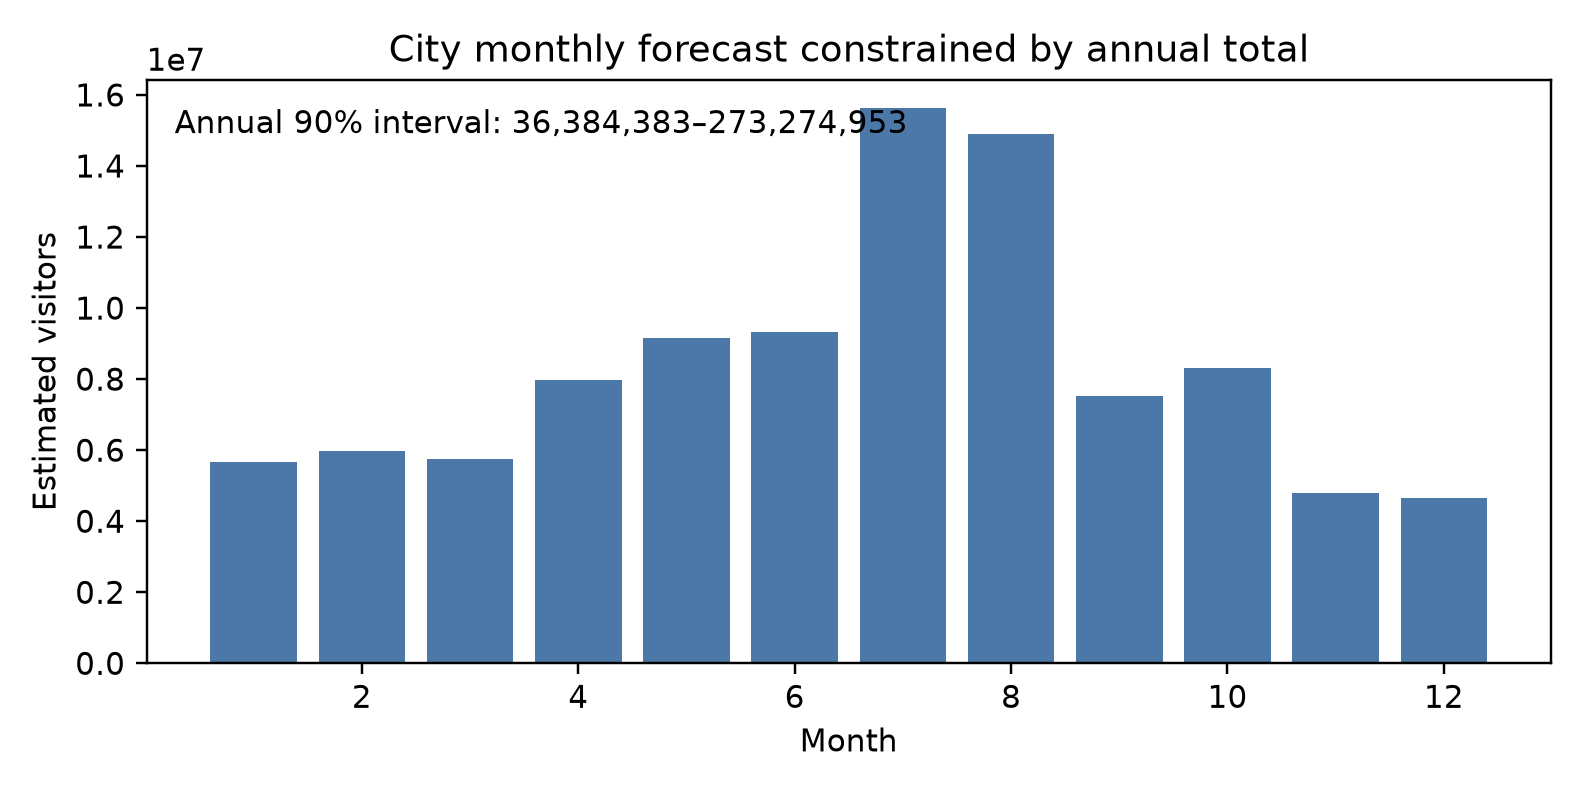
\includegraphics[width=.9\textwidth]{q2_city_monthly_forecast.png}\caption{全市月度预测}\end{figure}
\section{三区日级预测}
以2024年149条去重“片区--日期”观测作为完全留出集（2025年仅14条，不参与筛选）。目的地搜索仅在预测期前的真实观测日期中，从1、2、3、7日滞后按片区选择；北戴河、海港--阿那亚、山海关依次取1、3、2日。动态Ridge的MAE、RMSE、sMAPE为0.918、1.504、64.30\%，优于季节--日历Ridge的0.959、1.565、67.96\%，故作为日级基准。仅用2023年184条观测进行区域split-conformal校准后，三区半径依次为0.592、0.670、1.572；山海关半径大于1，故其下界截断为零并明确解释为高不确定性警示，而不是精确区间。暑期日峰值的三个分位数见表\ref{tab:q2peak}。
\begin{table}[H]\centering\caption{2026年暑期日峰值分位情景（人次）}\label{tab:q2peak}\begin{tabular}{lrrr}\toprule
片区&q10&q50&q90\\\midrule
北戴河&52\,041&127\,462&202\,883\\
海港--阿那亚&19\,230&58\,204&97\,179\\
山海关&0&135\,474&348\,466\\\bottomrule
\end{tabular}\end{table}
\begin{figure}[H]\centering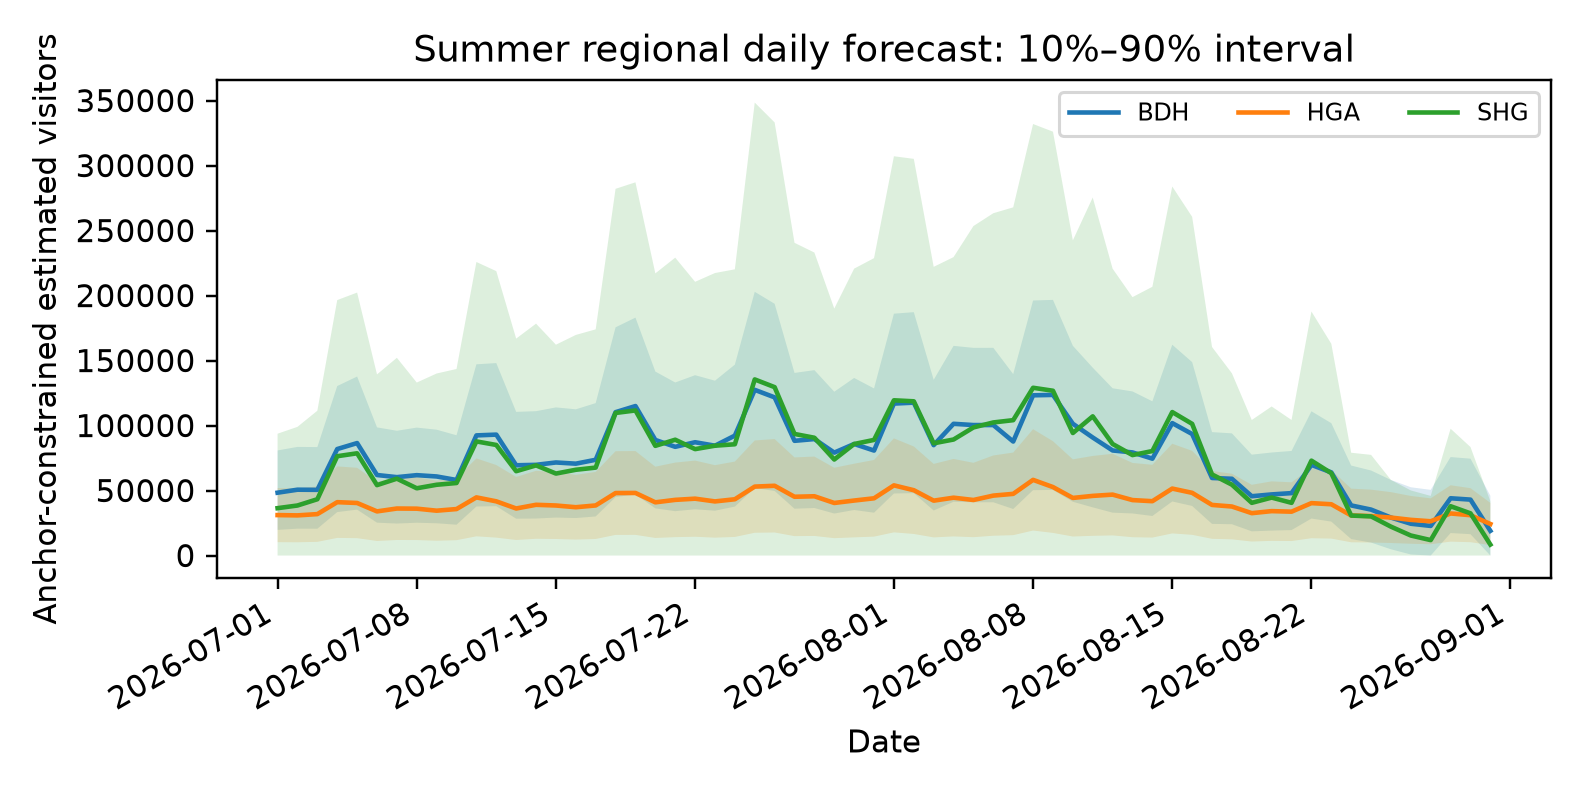
\includegraphics[width=.9\textwidth]{q2_summer_regional_daily_forecast.png}\caption{三大片区暑期日级预测}\end{figure}
\section{外部锚点与结论}
公开报道仅在统计范围一致时用于直接校验；景区或单一度假区的累计接待量与片区模型范围不一致时，仅作量级参照，不计算误差。问题二提供了全市年度规模、三区日级分位情景和天气扰动敏感性，供问题三、四在透明资源参数下使用。
\end{document}
